% Project 3 (Distributed control + HMI) - bản standalone
\documentclass[12pt,a4paper]{report}

\usepackage[utf8]{inputenc}
\usepackage[T5]{fontenc}
\usepackage{mathptmx}
\usepackage{amsmath}
\usepackage{graphicx}
\usepackage{float}
\usepackage{tikz}
\usetikzlibrary{calc,positioning}

\graphicspath{{docs/}{docs/figures/}{figures/}}

\begin{document}

% ====== TITLE PAGE ======
\begin{titlepage}
\centering
\vspace*{2cm}

{\Large \textbf{SPEC DỰ ÁN 3}\par}
\vspace{0.5cm}
{\LARGE \textbf{Mạng điều khiển phân tán và HMI (WiFi Mesh + LVGL)}\par}

\vspace{1.5cm}
{\large Tài liệu đặc tả kỹ thuật (Standalone)\par}

\vfill
{\large \today\par}
\end{titlepage}

\tableofcontents
\clearpage

% ====== MAIN CONTENT ======
\chapter{Dự án 3 --- Mạng điều khiển phân tán và HMI (WiFi Mesh + LVGL)}

\section{Mục tiêu và phạm vi}
Mục tiêu của kiến trúc phân tán là tách các node công suất/đo lường khỏi node hiển thị để tăng chống nhiễu, dễ mở rộng và quản lý tập trung. Ở phiên bản này, hệ thống sử dụng \textbf{WiFi mesh ESP32} (ESP-MESH) thay cho CAN bus: một node gốc (root) đóng vai trò gateway lên Wi-Fi/Cloud và điều phối, nhiều node con (Peltier, Bơm, HMI) tham gia mesh để gửi telemetry và nhận lệnh điều khiển. Node HMI dùng LVGL để hiển thị và cho phép đặt ngưỡng/chế độ thông qua mesh.

\section{Topology hệ thống (sơ đồ khối)}

\begin{figure}[H]
\centering
\resizebox{\textwidth}{!}{%
\begin{tikzpicture}[
  node distance=12mm,
  block/.style={draw, rounded corners, align=center, minimum width=26mm, minimum height=10mm},
  arrow/.style={->, thick},
  mesh/.style={<->, thick, dashed}
]
  \node[block] (root) {Root node\\ESP32 Mesh\\+ Gateway/Backend};
  \node[block, below left=18mm and 0mm of root] (node1) {Node Peltier\\(Project 1)};
  \node[block, below=18mm of root] (node2) {Node Bơm\\(Project 2)};
  \node[block, below right=18mm and 0mm of root] (hmi) {Node HMI\\LCD/TFT + LVGL};

  % liên kết mesh giữa root và các node
  \draw[mesh] (root) -- node[right]{Mesh link} (node1);
  \draw[mesh] (root) -- (node2);
  \draw[mesh] (root) -- (hmi);

  % một vài liên kết mesh chéo minh hoạ
  \draw[mesh] (node1) -- (node2);
  \draw[mesh] (node2) -- (hmi);
\end{tikzpicture}%
}
\caption{Topology hệ thống WiFi mesh nhiều node ESP32 và HMI}
\label{fig:p3_topology}
\end{figure}

\begin{figure}[H]
\centering
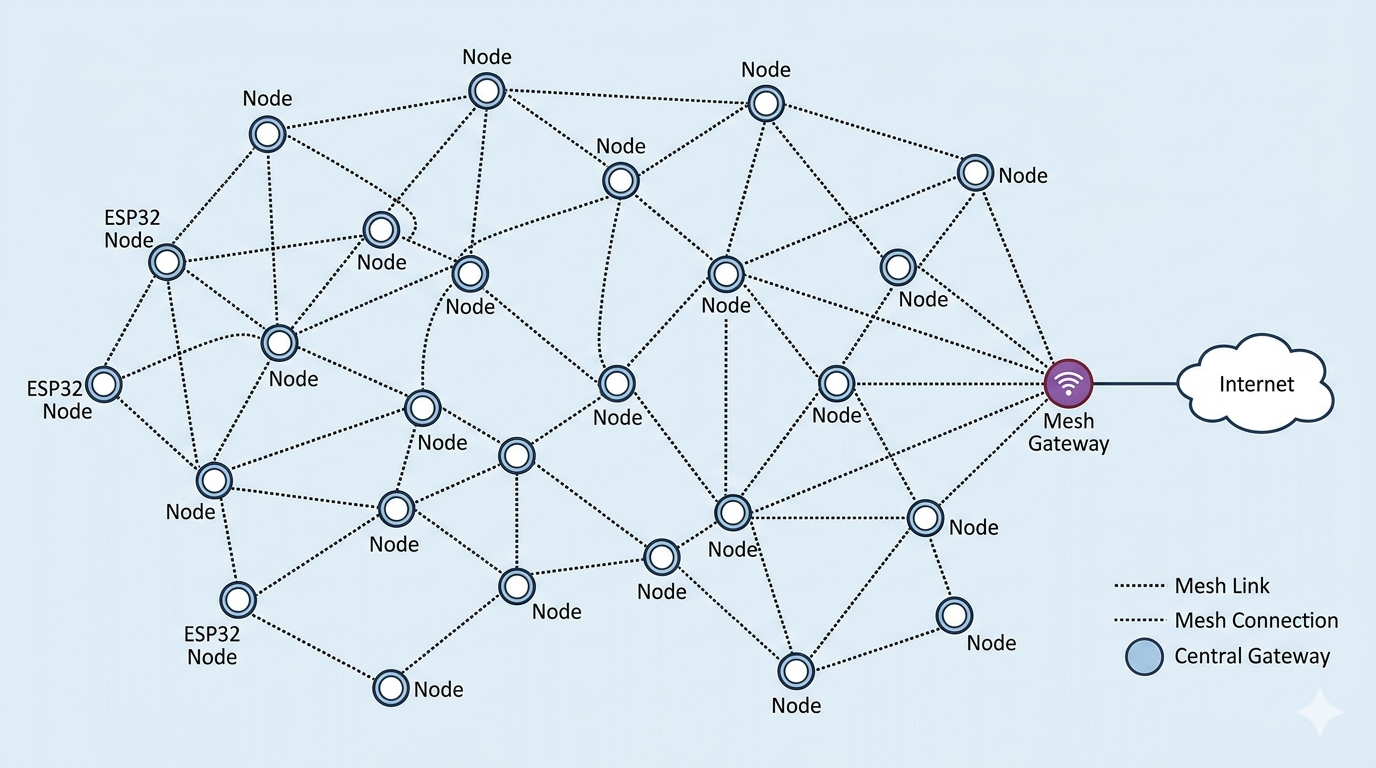
\includegraphics[width=0.85\textwidth]{figures/p3_mesh_topology.png}
\caption{Sơ đồ mesh WiFi nhiều node ESP32: các node được nối với nhau bằng các liên kết mesh, một node đóng vai trò gateway nối ra Internet/backend.}
\label{fig:p3_mesh_topology_img}
\end{figure}

\section{Yêu cầu phần cứng và giao tiếp}
\begin{itemize}
  \item \textbf{Mỗi node}: ESP32 (có WiFi) + nguồn 12V và buck xuống 5V/3.3V tuỳ phần công suất đi kèm (Peltier, Bơm, HMI).
  \item \textbf{Kết nối mesh}: anten WiFi tốt (anten PCB hoặc anten ngoài nếu khoảng cách xa), bố trí tránh che chắn bởi kim loại.
  \item \textbf{Gateway}: root node có kết nối Wi-Fi STA hoặc Ethernet (qua module bổ sung) để uplink cloud/backend (tuỳ chọn).
\end{itemize}

\begin{figure}[H]
\centering
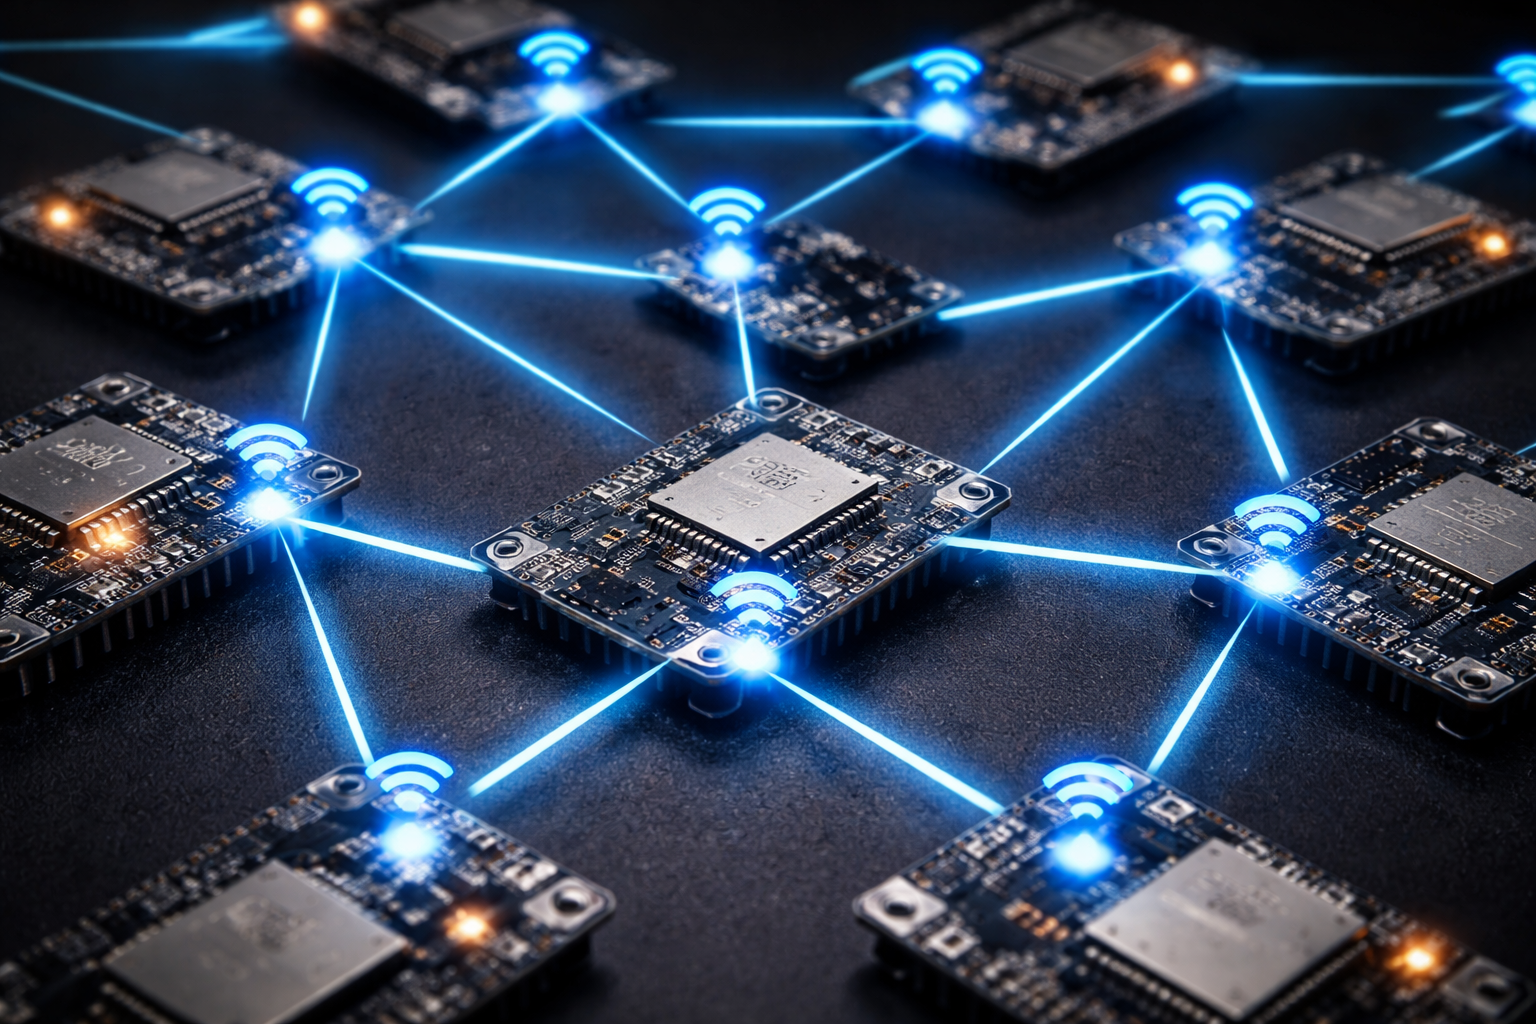
\includegraphics[width=0.85\textwidth]{figures/p3_mesh_boards.png}
\caption{Ảnh minh hoạ nhiều board ESP32 trong một mạng mesh, mỗi board đóng vai trò một node đo lường hoặc chấp hành trong hệ thống.}
\label{fig:p3_mesh_boards}
\end{figure}

\begin{figure}[H]
\centering
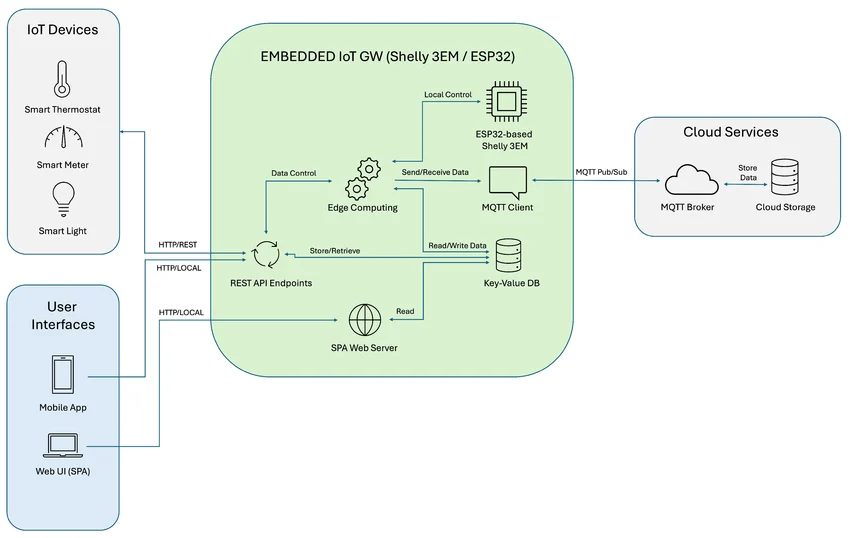
\includegraphics[width=0.85\textwidth]{figures/p3_gateway_architecture.jpg}
\caption{Kiến trúc gateway IoT dựa trên ESP32: gateway thu thập dữ liệu từ các thiết bị/mesh node, xử lý cục bộ và gửi dữ liệu lên dịch vụ cloud qua MQTT/HTTP.}
\label{fig:p3_gateway_architecture}
\end{figure}

\section{Bảng I/O tối thiểu (Root/HMI/Node công suất)}

\begin{table}[H]
\centering
\caption{I/O và giao tiếp tối thiểu --- Dự án 3 (WiFi mesh)}
\begin{tabular}{|p{3.0cm}|p{3.0cm}|p{3.0cm}|p{6.0cm}|}
\hline
\textbf{Node} & \textbf{Giao tiếp} & \textbf{Tín hiệu} & \textbf{Ghi chú}\\
\hline
Root (Gateway) & WiFi STA/AP & SSID/PASS mesh, uplink WiFi & Khởi tạo ESP-MESH, làm root, uplink backend\\
\hline
Root (Gateway) & UART (tuỳ chọn) & TX/RX & Logging, debug, cấu hình tại chỗ\\
\hline
Node công suất & WiFi mesh & Mesh link tới root/các node & Nhận lệnh điều khiển, gửi telemetry Peltier/Bơm\\
\hline
HMI & WiFi mesh + SPI/I2C (LCD/touch) & Mesh link + giao tiếp LCD & LVGL; cập nhật hiển thị và gửi lệnh qua mesh\\
\hline
\end{tabular}
\end{table}

\section{Đặc tả bản tin trên mesh WiFi}
Ở tầng logic, các node trao đổi với nhau bằng các bản tin JSON ngắn truyền qua ESP-MESH (unicast hoặc broadcast tuỳ loại message). Root đóng vai trò hub tiếp nhận mọi telemetry và phân phối lệnh tới các node con.

\subsection{Các loại bản tin chính}
\begin{itemize}
  \item \textbf{Telemetry Peltier} (\texttt{telemetry\_peltier}): Node Peltier $\rightarrow$ Root, chứa $T/H$, trạng thái Peltier, lỗi.
  \item \textbf{Telemetry Pump} (\texttt{telemetry\_pump}): Node Bơm $\rightarrow$ Root, chứa PWM, dòng $I$, mode, lỗi.
  \item \textbf{Command Peltier} (\texttt{cmd\_peltier}): Root $\rightarrow$ Node Peltier, thiết lập ngưỡng $T/H$, enable, tham số an toàn.
  \item \textbf{Command Pump} (\texttt{cmd\_pump}): Root $\rightarrow$ Node Bơm, thiết lập mode, PWM set, $I_{set}$, $I_{max}$, enable.
  \item \textbf{HMI Update} (\texttt{hmi\_update}): Root $\rightarrow$ HMI, gửi dữ liệu tổng hợp để hiển thị (T/H, dòng, trạng thái thiết bị).
  \item \textbf{HMI Command} (\texttt{hmi\_command}): HMI $\rightarrow$ Root, gửi thao tác người dùng (thay đổi setpoint/mode, start/stop đo, v.v.).
\end{itemize}

\subsection{Ví dụ cấu trúc payload JSON}
Ví dụ một số payload (định dạng JSON). Mỗi mẫu được xuống dòng cho dễ đọc, vẫn có thể copy nguyên khối:

\begin{description}
  \item[\textbf{Telemetry Peltier}]
  \begin{verbatim}
{"type":"telemetry_peltier",
 "deviceId":"peltier-1",
 "temp":24.8,
 "hum":62.1,
 "status":"ok"}
  \end{verbatim}

  \item[\textbf{Telemetry Pump}]
  \begin{verbatim}
{"type":"telemetry_pump",
 "deviceId":"pump-1",
 "pwm":60,
 "current":0.45,
 "mode":"AUTO",
 "status":"ok"}
  \end{verbatim}

  \item[\textbf{Command Peltier}]
  \begin{verbatim}
{"type":"cmd_peltier",
 "deviceId":"peltier-1",
 "t_min":20,
 "t_max":25,
 "h_min":60,
 "h_max":65,
 "enable":true}
  \end{verbatim}

  \item[\textbf{Command Pump}]
  \begin{verbatim}
{"type":"cmd_pump",
 "deviceId":"pump-1",
 "mode":"AUTO",
 "I_set":0.4,
 "I_max":0.8,
 "enable":true}
  \end{verbatim}

  \item[\textbf{HMI Command}]
  \begin{verbatim}
{"type":"hmi_command",
 "action":"set_setpoint",
 "t_max":25,
 "h_max":65}
  \end{verbatim}
\end{description}

\section{Yêu cầu cơ khí và bố trí (bổ sung)}
Để tài liệu triển khai rõ ràng, ngoài các yêu cầu riêng cho từng node (đã nêu ở các dự án 1 và 2), hệ thống mesh cần lưu ý thêm:
\begin{itemize}
  \item \textbf{Vị trí node}: bố trí các node sao cho vẫn nằm trong vùng phủ WiFi ổn định (RSSI đủ cao), tránh đặt anten sát kim loại hoặc trong hộp kín hoàn toàn.
  \item \textbf{Nguồn cấp}: đường cấp 12V và buck xuống 5V/3.3V cho từng node cần tách mass hợp lý để hạn chế nhiễu lên RF.
  \item \textbf{HMI}: xác định vị trí màn hình, lỗ bắt vít, hướng cáp FPC và đường dây tới board ESP32 để tránh gây nhiễu cho anten.
\end{itemize}

\section{Fail-safe và độ tin cậy}
\begin{itemize}
  \item \textbf{Timeout mesh}: mỗi node công suất về trạng thái an toàn nếu không nhận được lệnh/heartbeat từ root trong $t_{timeout}$ (gợi ý 3--5s).
  \item \textbf{Mất root hoặc phân tách mạng}: cân nhắc cấu hình root cố định; nếu root mất nguồn, tất cả node công suất phải tắt Peltier/bơm hoặc về chế độ an toàn.
  \item \textbf{Restart node}: khi node khởi động lại, phải gia nhập mesh, đăng ký lại và chỉ bật công suất sau khi nhận cấu hình hợp lệ từ root.
  \item \textbf{Checksum/sequence (tuỳ chọn)}: thêm trường \texttt{seq} trong payload để phát hiện mất gói/lặp gói trên tầng ứng dụng.
\end{itemize}

\end{document}
